% sections/07_results.tex

\section{Experimental Results}

% --- Slide 1: Hardware Specs ---
\begin{frame}{Experimental Results: Hardware Specifications}
  \begin{columns}[onlytextwidth, T]
    \column{0.6\textwidth}
      \begin{itemize}
        \item \textbf{PC Build (Workstation):} 
        \begin{itemize}
          \item \textbf{CPU:} Intel Xenon CPU E5-2620@2.10 GHz with 24 cores \textit{(Inferred Dual-Processor setup)}.
          \item \textbf{RAM:} 16 GB DDR3 \textit{(Inferred Quad-Channel configuration)}.
          \item \textbf{Storage:} 1 TB of disk storage \textit{(Inferred HDD for HDFS layer)}.
        \end{itemize}
      \end{itemize}

    \column{0.4\textwidth}
      \centering
      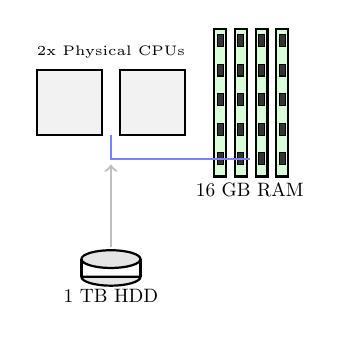
\begin{tikzpicture}[scale=0.75]
        \draw[thick, fill=gray!10] (0,1.2) rectangle (1.1,2.3);
        \draw[thick, fill=gray!10] (1.4,1.2) rectangle (2.5,2.3);
        \node at (1.25,2.6) {\tiny 2x Physical CPUs};

        \foreach \x in {0, 0.35, 0.7, 1.05} {
          \draw[thick, fill=green!15] (3.0+\x, 0.5) rectangle (3.0+\x+0.2, 3);
          \foreach \y in {0.7, 1.2, 1.7, 2.2, 2.7}
            \draw[fill=black!80] (3.0+\x+0.05, \y) rectangle (3.0+\x+0.15, \y+0.2);
        }
        \node[below, scale=0.7] at (3.6,0.5) {16 GB RAM};
        
        \begin{scope}[yshift=-1.2cm, xshift=1.25cm]
            \draw[thick, fill=gray!20] (0,0.3) ellipse (0.5 and 0.15);
            \draw[thick] (-0.5,0) -- (-0.5,0.3);
            \draw[thick] (0.5,0) -- (0.5,0.3);
            \draw[thick, fill=gray!20] (-0.5,0) arc (180:360:0.5 and 0.15) -- (0.5,0) -- cycle;
            \node[below, scale=0.7] at (0,-0.1) {1 TB HDD};
        \end{scope}
        
        \draw[thick, blue!50] (1.25,1.2) -- (1.25,0.8) -- (3.6,0.8);
        \draw[thick, gray!50, ->] (1.25,-0.7) -- (1.25,0.7);
      \end{tikzpicture}
  \end{columns}

  \vfill
  \begin{alertblock}{Hardware Capacity}
    The dual-processor setup provides 24 execution threads, while the quad-channel memory configuration ensures high data transfer speeds between the RAM and the CPUs.
  \end{alertblock}
\end{frame}

% --- Slide 2: Software Stack ---
\begin{frame}{Experimental Results: Software \& Memory Mode}
  \begin{columns}[onlytextwidth, T]
    \column{0.6\textwidth}
      \begin{itemize}
        \item \textbf{Software Stack:} 
        \begin{itemize}
          \item \textbf{OS:} Ubuntu 14.04 (64-bit).
          \item \textbf{Frameworks:} Spark 2.1.1, Hadoop 2.6.0.
          \item \textbf{Language:} Java 7 / Scala 2.11.8.
        \end{itemize}
        \vfill
        \item \textbf{Memory Mode:} 
        \begin{itemize}
          \item \textbf{Level:} \texttt{MEMORY\_ONLY}.
          \item \textbf{Strategy:} RDDs are cached in RAM.
          \item \textbf{Impact:} Bypasses Disk I/O bottlenecks during $L_k$ generation.
        \end{itemize}
      \end{itemize}

    \column{0.4\textwidth}
      \centering
      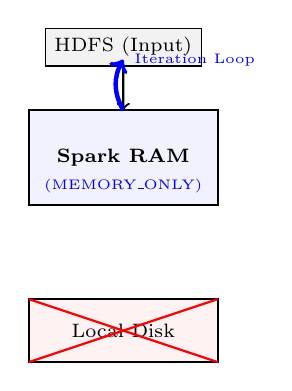
\begin{tikzpicture}[scale=0.8]
        \node[draw, fill=gray!10] (hdfs) at (1.5,4) {\scriptsize HDFS (Input)};
        \draw[thick, fill=blue!5] (0,1.5) rectangle (3,3);
        \node at (1.5,2.25) {\scriptsize \textbf{Spark RAM}};
        \node[blue] at (1.5,1.8) {\tiny (MEMORY\_ONLY)};
        \draw[thick, fill=red!5] (0,0) rectangle (3,-1);
        \node at (1.5,-0.5) {\scriptsize Local Disk};
        \draw[red, thick] (0,0) -- (3,-1); \draw[red, thick] (3,0) -- (0,-1);
        \draw[->, thick] (hdfs) -- (1.5,3);
        \draw[->, blue, ultra thick] (1.5,3) to [bend left] (1.5,3.8) node[right] {\tiny Iteration Loop};
      \end{tikzpicture}
  \end{columns}
\end{frame}

% --- Slide 3: Performance I (2x2 Plot - Mushroom/Chess) ---
\begin{frame}{Performance Analysis: Datasets (a) to (d)}
    \vspace{-0.2cm}
    \begin{center}
        
\includegraphics[height=0.72\textheight, width=0.95\textwidth, keepaspectratio]{plots_2x2.png}
    \end{center}
    \vspace{-0.3cm}
    \begin{itemize}
        \item \footnotesize \textbf{Observation:} On dense datasets like \textit{Mushroom} and \textit{Chess}, HTT maintains a steady \textbf{2x speedup} by optimizing CPU cache usage during RDD lookups.
    \end{itemize}
\end{frame}

% --- Slide 4: Performance II (Triangular Plot - BMS) ---
\begin{frame}{Performance Analysis: Datasets (e) to (g)}
    \vspace{-0.2cm}
    \begin{center}
        
\includegraphics[height=0.72\textheight, width=0.95\textwidth, keepaspectratio]{plots_triangular.png}
    \end{center}
    \vspace{-0.3cm}
    \begin{itemize}
        \item \footnotesize \textbf{Observation:} For sparse datasets (BMS1/BMS2), the efficiency of the Trie-based architecture becomes even more apparent, achieving an \textbf{8x performance gain}.
    \end{itemize}
\end{frame}

% --- Slide 5: Summary Table ---
\begin{frame}{Experimental Results: Summary Table}
    \centering
    \begin{beamercolorbox}[sep=6pt,center,rounded=true]{block body}
        \textbf{Relative Speedup vs. Hash Tree (HT)}
    \end{beamercolorbox}
    \vspace{0.1cm}
    \begin{tabular}{|l|c|c|c|}
        \hline
        \textbf{Dataset} & \textbf{HT (Baseline)} & \textbf{Trie} & \textbf{HTT} \\ \hline
        BMS1 / BMS2      & 1.0x                & \textbf{> 8.0x} & \textbf{> 8.0x} \\ \hline
        T40I10D100K      & 1.0x                & 5.8x            & \textbf{6.1x}   \\ \hline
        Mushroom / Chess & 1.0x                & 1.9x            & \textbf{2.1x}   \\ \hline
    \end{tabular}
    \vfill
    \begin{alertblock}{The RDD Conclusion}
        \small The results validate that within Spark, the computational efficiency of $O(1)$ lookups in the Hash Table Trie (HTT) justifies its memory footprint.
    \end{alertblock}
\end{frame}
